\documentclass[a4paper,12pt]{article}
\usepackage[brazil]{babel}
\usepackage[utf8]{inputenc}
\usepackage{amsthm}
\usepackage{amsfonts}
\usepackage{graphicx}
\begin{document}

\title{Condição de Imagem com Hadoop}
\author{Ian Liu Rodrigues -- 061485}
\maketitle

\begin{abstract}
  A \emph{condição de imagem} é uma etapa do algoritmo \emph{Migração em
  Tempo Reverso}, ou \emph{MTR}, cujo objetivo é criar um mapa de
  coerência de sinais coletados em campo.
\end{abstract}

\section{Introdução}

\subsection{Cubo de dados}

Um cubo de dados de tamanho $n_z \times n_x \times n_t$ representa um
filme da evolução de ondas acústicas se propagando em uma malha de
tamanho $n_z \times n_x$. Cada fatia do dado no plano $XZ$ representa
amplitudes de pressão num dado tempo $t$. Em disco, um cubo de dados
pode chegar a ocupar vários gigabytes.

Os cubos de dados são gerados por meios de simulações acústicas. O
método das diferenças finitas pode ser usado para realizar tais
simulações.

\begin{figure}
  \centering
  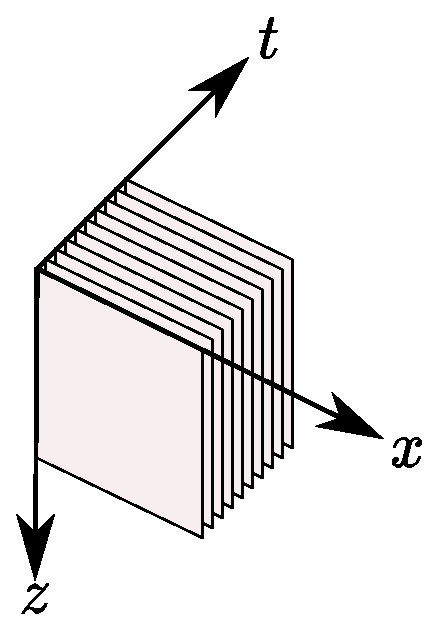
\includegraphics[width=3cm]{images/cubo-de-dados}
  \caption{Representação de um cubo de dados divididos em fatias de
  tempo.}
\end{figure}

\subsection{Fonte \& Receptores}

Uma fonte sísmica pode ser um explosivo que gera grandes pressões no
solo. Essas ondas de pressão se propagam na estrutura rochosa e são
refletidas quando encontram mudanças de solo, rupturas, etc. As
vibrações que chegam até a superfície são mensuradas pelos receptores.

\begin{figure}
  \centering
  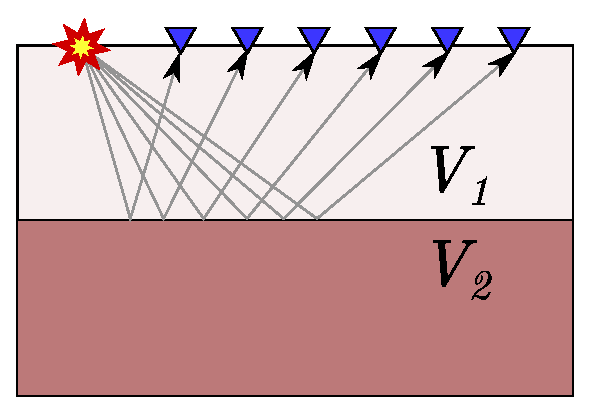
\includegraphics[width=6cm]{images/solo}
  \caption{A estrela amarela representa uma fonte, que propaga suas
  ondas acústicas até os receptores. A mudança do solo é caracterizada
pela velocidade em que as ondas acústicas viajam no meio.}
\end{figure}

\section{Condição de Imagem}

Uma simulação da propagação das ondas acústicas é realizada para cada
receptor e para a fonte. Cada simulação gera um cubo de dados, que serão
multiplicados ponto-a-ponto e somados, gerando uma imagem final. Por
exemplo, se temos a fonte $S(x, z, t)$ e os receptores $R_i(x, z, t)$,
definimos a seguinte imagem:
\[
  I(x, z) = \sum_t \sum_r S(x, z, t)R_r(x, z, t).
\]

\end{document}
